\section{Data Driven Background Estimation Methods}
\label{sec:datadriven}

We have developed two data-driven methods to 
estimate the two potentially dominant backgrounds.
The first method provides an estimate of the number of events with fake leptons (jets misidentified as leptons).
The second method is used to estimate the number of genuine leptons reconstructed with an incorrect charge sign.

\subsection{Data Driven prediction for fake lepton backgrounds}
\label{sec:fakes}

We predict the background from fake leptons using the technique previously implemented in 2010 data analysis
and documented in~\cite{frmethod}.
The idea is to count the number of events for which one lepton passes all final selections and a second lepton
fails the nominal requirements but passes a looser set of requirements. 
We refer to the former lepton as a "numerator" lepton ($n$),
and the latter a "non-numerator" (denominator and not numerator, or $\bar{n}$).
The denominator objects are also referred to as fakeable objects (FO).
The ratio of "numerator" to "denominator" objects is called a "fake rate",
 FR (also known as tight-to-loose ratio, TL).  
A fake rate function is measured in an independent data sample of multijet events.
This fake rate function is measured in bins of lepton $\pt$ and $|\eta |$,
separately for electrons and muons. 

The numerator selections are detailed in Section~\ref{sec:eventSel}. 
The denominator selections are described below, specifying only looser selections.

Muon denominator definition is to relax the following muon requirements from
Section~\ref{sec:eventSel}:
\begin{itemize}
\item $\chi^2$/ndof of global fit $<$ 50 (was $<$ 10);
\item transverse impact parameter with respect to the selected vertex is
$<$ 2 mm (was $<$ 200 $\mu$m);
\item $Iso$ is set to be $Iso < 0.4$  (was $<$ 0.1).
\end{itemize}

Electron denominator definition is to relax the following electron requirements from
Section~\ref{sec:eventSel}:
\begin{itemize}
\item the impact parameter cut is removed (was $<$ 200 $\mu$m);
\item $Iso$ is set to be $Iso < 0.6$ (was $<0.10$).
\end{itemize}
This is analogous to the V3 denominator in~\cite{frmethod} used for our previous analysis.

We thus use an extrapolation  in isolation (and impact parameter) to estimate the fake lepton backgrounds 
in both electrons and muons.
This choice is driven by the expectation that the selected events with fake leptons are dominated by
heavy flavor jets, in which the lepton candidate is predominantly a real lepton from b/c-quark semileptonic decays.
Relaxed isolation and impact parameter selections are then expected to roughly keep the same sample
composition in events with denominator leptons.

Samples of multijet (inclusive QCD) events in data are selected among events with a single lepton trigger present.
The samples and the triggers used in this measurement are listed in Section~\ref{sec:datasets}.
Since essentially all of the dilepton analysis events are collected on dilepton-triggered events, the
most appropriate choice for the FR measurement is to use  triggers based on the same (or almost the same) 
single-object triggers as the signal selection dilepton triggers.
The single-lepton triggered events are required to have an electron or a muon passing the denominator
requirements described above.
These events are further pruned of the contamination from the electroweak processes with W or Z production.
The W events are suppressed by a requirement that \met is below 20~GeV and the transverse mass $M_T < 25$~GeV.
The Z events are initially suppressed
by removing dielectron and dimuon events with another lepton matching 
the fakeable object and forming a pair with an invariant mass within the 71 to 111~GeV range
(events are removed only with  dileptons with both $\pt>20$~GeV and the other lepton
 passing a looser ID and isolation selection of the early $t\bar{t}$ analysis~\cite{frmethod}).
Further stringent suppression of remaining Z events is achieved by vetoing events satisfying the following conditions,
\begin{itemize}
\item for electrons:
\begin{itemize}
  \item other fakeable objects with $\pt>10~\GeV$ are present;
  \item there is a GSF track making a pair with the fakeable object and an invariant mass of 76 -- 106~GeV;
  \item the away jet has an EM-fraction higher than 0.8. 
\end{itemize}
\item for muons:
\begin{itemize}
  \item other fakeable objects with $\pt>10~\GeV$ are present;
  \item there is another muon (no ID requirement) with $\pt>10~\GeV$ making a pair with the fakeable object with an invariant mass of 76 -- 106~GeV;
  \item there is another muon (no ID requirement) with $\pt>10~\GeV$ making a pair with the fakeable object with an invariant
  mass between 8 and 12~GeV to additionally suppress Upsilon production contribution.
\end{itemize}
\end{itemize}

We repeat all the studies performed with 2010 data, as documented in~\cite{frmethod}.
These include 
\begin{itemize}
\item extraction of the fake rates in simulation and data;
\item closure tests on W+jet, \ttbar, and double-fake QCD events;
\item measurement of the fake-rate dependence on the {\em opposite-side} jet \pt,
	as a measure of the dependence on the progenitor parton momentum;
\item estimates of the residual W+jet and Z contamination in the sample;
\item comparison with the fake rate measured in events with enhanced heavy flavor
	contribution using b-tagging (the variation observed here is up to about 20\% for electrons and
	muons in both simulation and data).
\end{itemize}
We arrive to essentially the same conclusions on the performance of the fake-rate method
as we did in the past.
In particular, we find that the method works reasonably well, still with a systematic
uncertainty of about 50\%.
In the following we summarize the measurement of the fake rate and provide several highlights
of the studies with the current dataset.

The nominal fake rates are measured requiring an "opposite side" jet with $\pt>40~\GeV$, 
separated by $\Delta R > 1.0$ from the FO.
The electron fake rates are measured separately for triggers with an isolation requirement and
for triggers without any isolation requirement on the electron.
Results of the measurement are summarized in Tables~\ref{tab:frelectronTCaloIso},~\ref{tab:frelectronTNoIso} and ~\ref{tab:frelectronTCaloIsoTrkIso}
for the case with calorimeter, without, and with calorimeter and tracker isolation requirements, respectively.
The muon fake rates are measured using all single-muon triggers described in Section~\ref{sec:datasets}.
The measurement is summarized in Table~\ref{tab:frmuon}.


\begin{table}[h]
\begin{center}
\begin{tabular}{c|ccccc}
\hline
\backslashbox{$|\eta|$}{$p_T$} & 10.000 -- 15.000 & 15.000 -- 20.000 & 20.000 -- 25.000 & 25.000 -- 35.000 & 35.000 -- 55.000 \\ \hline\hline
0.000 -- 1.000 & 0.1985 $\pm$ 0.0141 & 0.1535 $\pm$ 0.0177 & 0.1260 $\pm$ 0.0212 & 0.1567 $\pm$ 0.0247 & 0.2198 $\pm$ 0.0434 \\ \hline
1.000 -- 1.479 & 0.1951 $\pm$ 0.0253 & 0.1867 $\pm$ 0.0318 & 0.1870 $\pm$ 0.0352 & 0.1800 $\pm$ 0.0384 & 0.3333 $\pm$ 0.0624 \\ \hline
1.479 -- 2.000 & 0.1880 $\pm$ 0.0339 & 0.1696 $\pm$ 0.0355 & 0.1481 $\pm$ 0.0279 & 0.1548 $\pm$ 0.0279 & 0.2596 $\pm$ 0.0430 \\ \hline
2.000 -- 2.500 & 0.2583 $\pm$ 0.0356 & 0.3084 $\pm$ 0.0446 & 0.1797 $\pm$ 0.0339 & 0.2836 $\pm$ 0.0389 & 0.3191 $\pm$ 0.0481 \\ \hline
\end{tabular}
\caption{\label{tab:frelectronTNoIso}Electron fake rate measured in bins of the electron candidate \pt\ and $\eta$
for electrons collected using triggers without isolation requirements.}
\end{center}
\end{table}

\begin{table}[htb]
\begin{center}
\begin{tabular}{c|ccccc}
\hline
\backslashbox{$|\eta|$}{$p_T$} & 10.000 -- 15.000 & 15.000 -- 20.000 & 20.000 -- 25.000 & 25.000 -- 35.000 & 35.000 -- 55.000 \\ \hline\hline
0.000 -- 1.000 & 0.2773 $\pm$ 0.0072 & 0.1784 $\pm$ 0.0072 & 0.1759 $\pm$ 0.0079 & 0.1789 $\pm$ 0.0084 & 0.2583 $\pm$ 0.0148 \\ \hline
1.000 -- 1.479 & 0.2749 $\pm$ 0.0121 & 0.2177 $\pm$ 0.0132 & 0.1977 $\pm$ 0.0115 & 0.1924 $\pm$ 0.0117 & 0.3026 $\pm$ 0.0197 \\ \hline
1.479 -- 2.000 & 0.2415 $\pm$ 0.0152 & 0.1806 $\pm$ 0.0137 & 0.1871 $\pm$ 0.0099 & 0.1916 $\pm$ 0.0095 & 0.2379 $\pm$ 0.0135 \\ \hline
2.000 -- 2.500 & 0.2827 $\pm$ 0.0146 & 0.2607 $\pm$ 0.0156 & 0.2420 $\pm$ 0.0119 & 0.2561 $\pm$ 0.0116 & 0.3225 $\pm$ 0.0154 \\ \hline
\end{tabular}
\caption{\label{tab:frelectronTCaloIso}Electron fake rate measured in bins of the electron candidate \pt\ and $\eta$
for electrons collected using triggers with a calorimeter isolation requirement.}
\end{center}
\end{table}

\begin{table}[htb]
\begin{center}
\begin{tabular}{c|ccccc}
\hline
\backslashbox{$|\eta|$}{$p_T$} & 10.000 -- 15.000 & 15.000 -- 20.000 & 20.000 -- 25.000 & 25.000 -- 35.000 & 35.000 -- 55.000 \\ \hline\hline
0.000 -- 1.000 & 0.3783 $\pm$ 0.0218 & 0.2932 $\pm$ 0.0279 & 0.2365 $\pm$ 0.0298 & 0.2713 $\pm$ 0.0324 & 0.3690 $\pm$ 0.0527 \\ \hline
1.000 -- 1.479 & 0.3556 $\pm$ 0.0357 & 0.3617 $\pm$ 0.0496 & 0.2364 $\pm$ 0.0405 & 0.2353 $\pm$ 0.0460 & 0.4667 $\pm$ 0.0644 \\ \hline
1.479 -- 2.000 & 0.2326 $\pm$ 0.0372 & 0.1638 $\pm$ 0.0344 & 0.2000 $\pm$ 0.0332 & 0.2260 $\pm$ 0.0314 & 0.2793 $\pm$ 0.0426 \\ \hline
2.000 -- 2.500 & 0.3357 $\pm$ 0.0399 & 0.2736 $\pm$ 0.0433 & 0.2362 $\pm$ 0.0377 & 0.2681 $\pm$ 0.0377 & 0.3645 $\pm$ 0.0465 \\ \hline
\end{tabular}
\caption{\label{tab:frelectronTCaloIsoTrkIso}Electron fake rate measured in bins of the electron candidate \pt\ and $\eta$
for electrons collected using triggers with calorimeter and tracker isolation requirements.}
\end{center}
\end{table}

\begin{table}[htb]
\begin{center}
\begin{tabular}{c|ccccc}
\hline
\backslashbox{$|\eta|$}{$p_T$} & 5.000 -- 10.000 & 10.000 -- 15.000 & 15.000 -- 20.000 & 20.000 -- 25.000 & 25.000 -- 35.000 \\ \hline\hline
0.000 -- 1.000 & 0.2760 $\pm$ 0.0028 & 0.2127 $\pm$ 0.0024 & 0.1808 $\pm$ 0.0032 & 0.1541 $\pm$ 0.0043 & 0.1441 $\pm$ 0.0009 \\ \hline
1.000 -- 1.479 & 0.3119 $\pm$ 0.0042 & 0.2527 $\pm$ 0.0036 & 0.2100 $\pm$ 0.0048 & 0.1820 $\pm$ 0.0067 & 0.1770 $\pm$ 0.0015 \\ \hline
1.479 -- 2.000 & 0.3340 $\pm$ 0.0042 & 0.2694 $\pm$ 0.0037 & 0.2238 $\pm$ 0.0049 & 0.2197 $\pm$ 0.0072 & 0.2018 $\pm$ 0.0016 \\ \hline
2.000 -- 2.500 & 0.3343 $\pm$ 0.0061 & 0.2741 $\pm$ 0.0054 & 0.2174 $\pm$ 0.0071 & 0.2012 $\pm$ 0.0108 & 0.2150 $\pm$ 0.0027 \\ \hline
\end{tabular}
\caption{\label{tab:frmuon}Muon fake rate measured in bins of the muon candidate \pt\ and $\eta$.
The uncertainties are statistical only.}
\end{center}
\end{table}

Figures~\ref{fig:frmuon}  and~\ref{fig:frelectron}  show the projection on $\pt$ and $|\eta|$ of these fake rates
for electrons and muons, respectively.
Electron fake rates measured for triggers with an isolation requirement are slightly higher than those
for triggers without an isolation requirement, as expected.
The difference, even though it's not very large, is significant enough and we treat fake rates for these triggers
separately.
The dependence of the fake rates on the away-jet momentum is also shown on these figures.

\begin{figure}[h]
\begin{center}
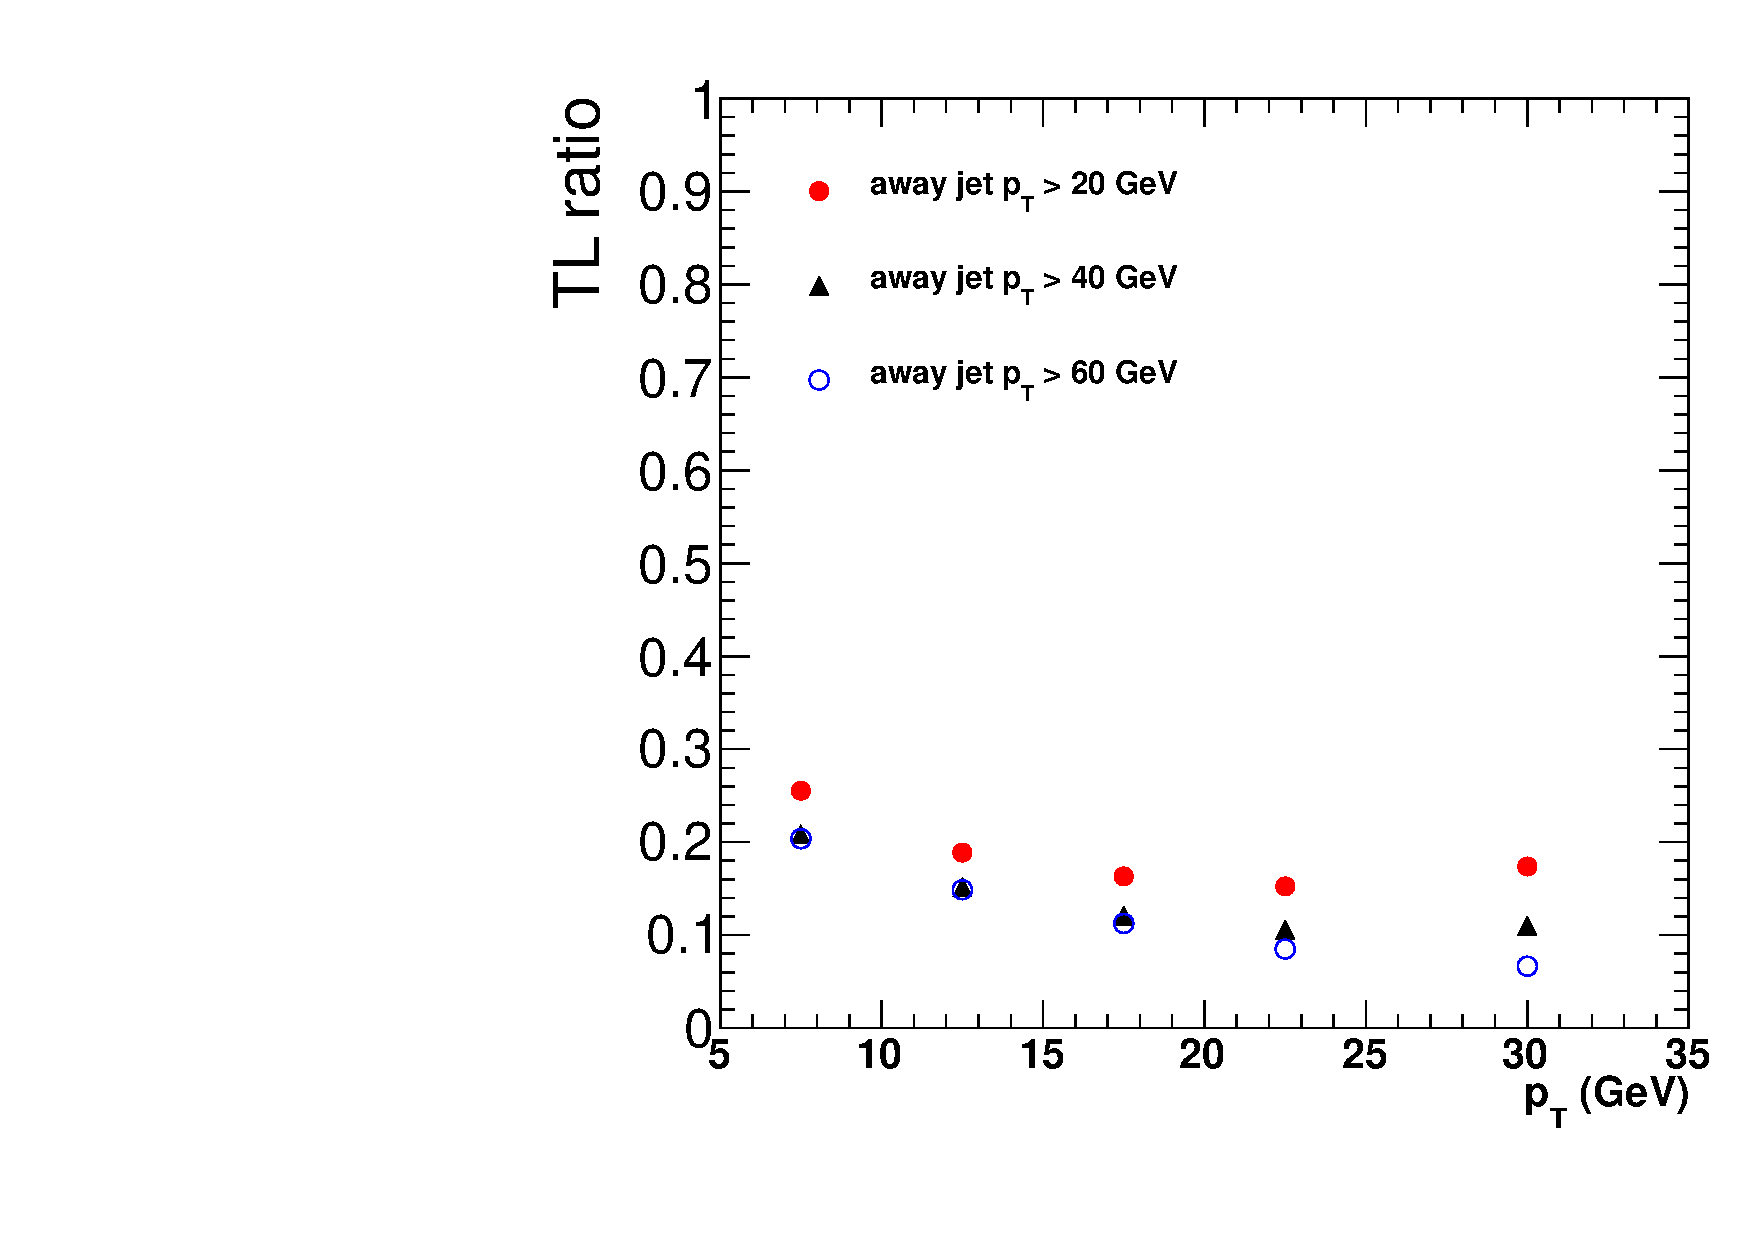
\includegraphics[width=0.48\linewidth]{figs/muFR_data_ptProj}
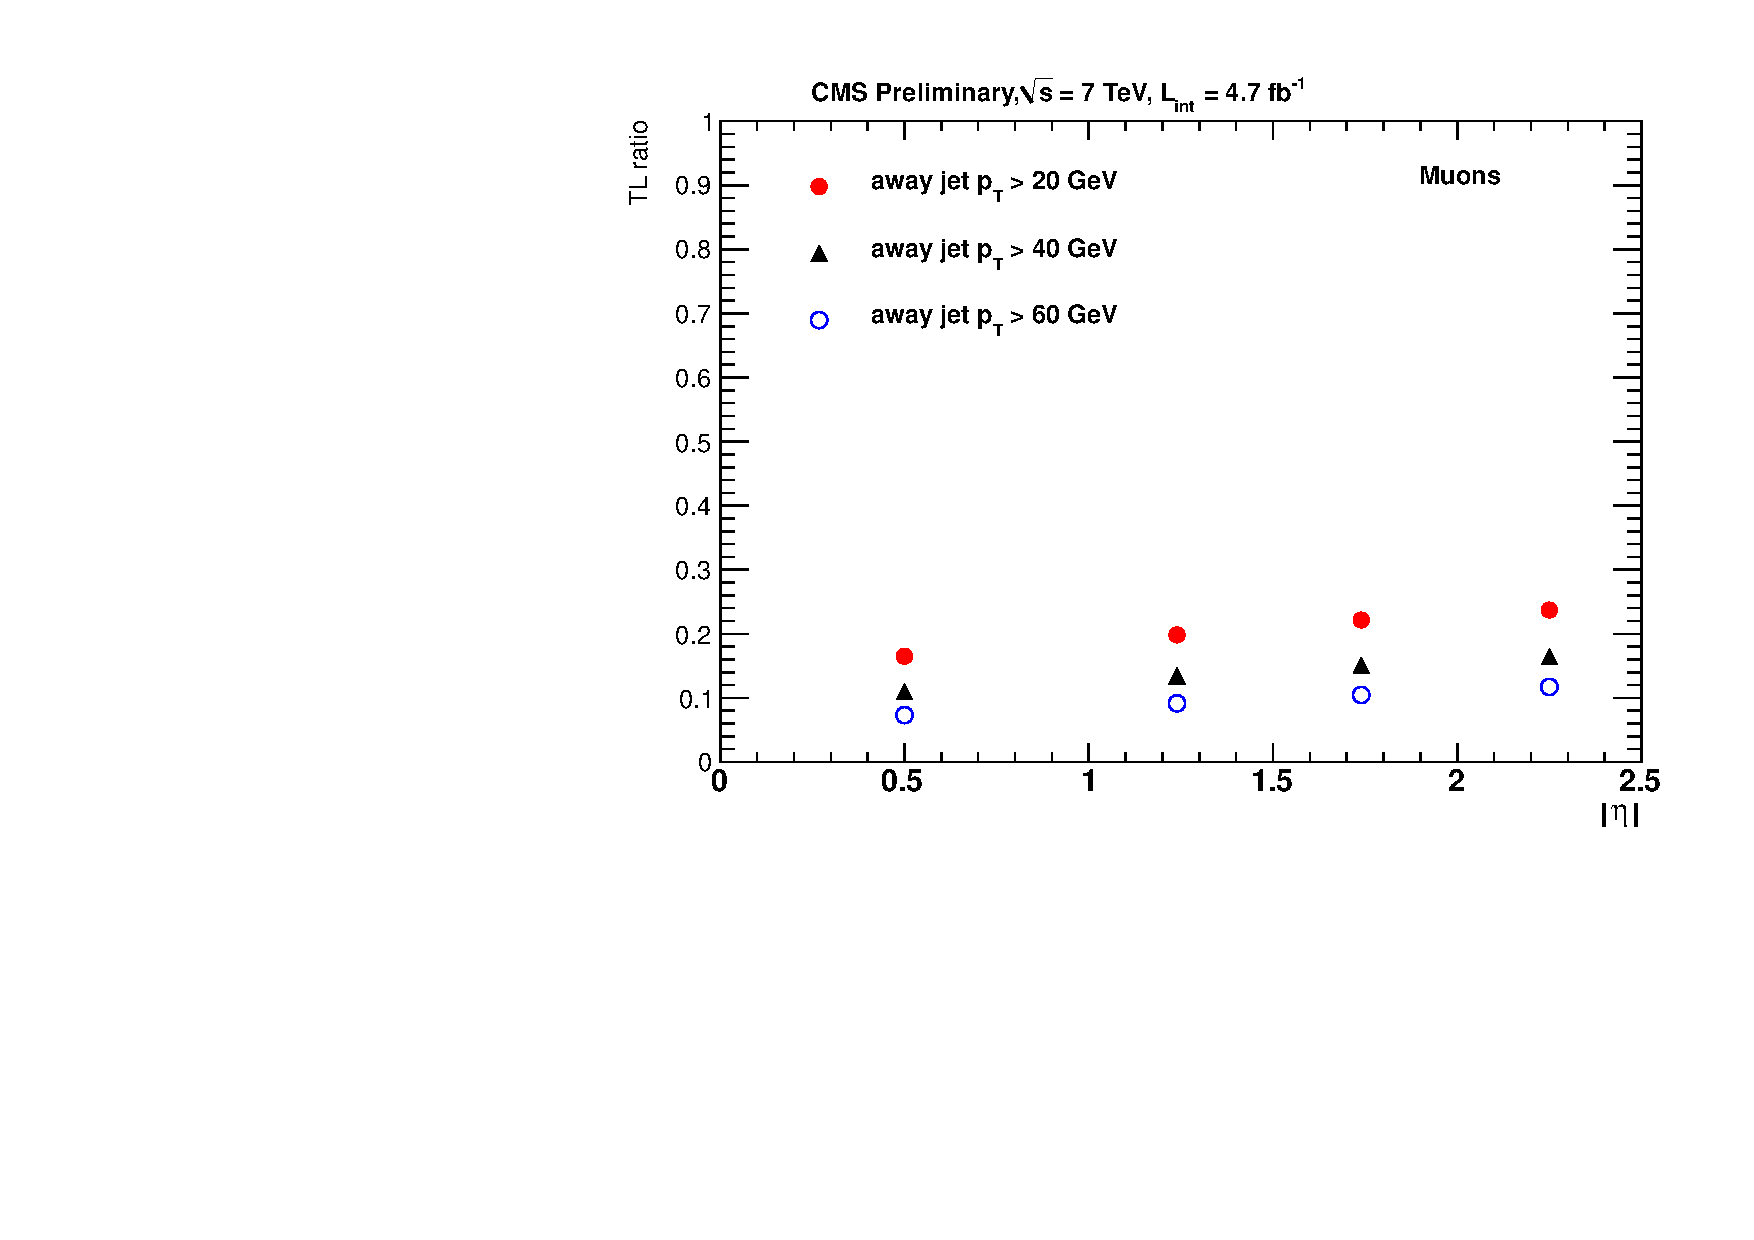
\includegraphics[width=0.48\linewidth]{figs/muFR_data_etaProj}
\caption{\label{fig:frmuon}Muon fake rate projected on $\pt$ (left) and $|\eta|$ (right).
The fake rates are shown separately for measurements  with a requirement for an away jet \pt\ 
to be above 20~\GeV\ (red circles), 40~\GeV\ (black circles), and 60~\GeV\ (blue circles).
}
\end{center}
\end{figure}

\begin{figure}[h]
\begin{center}
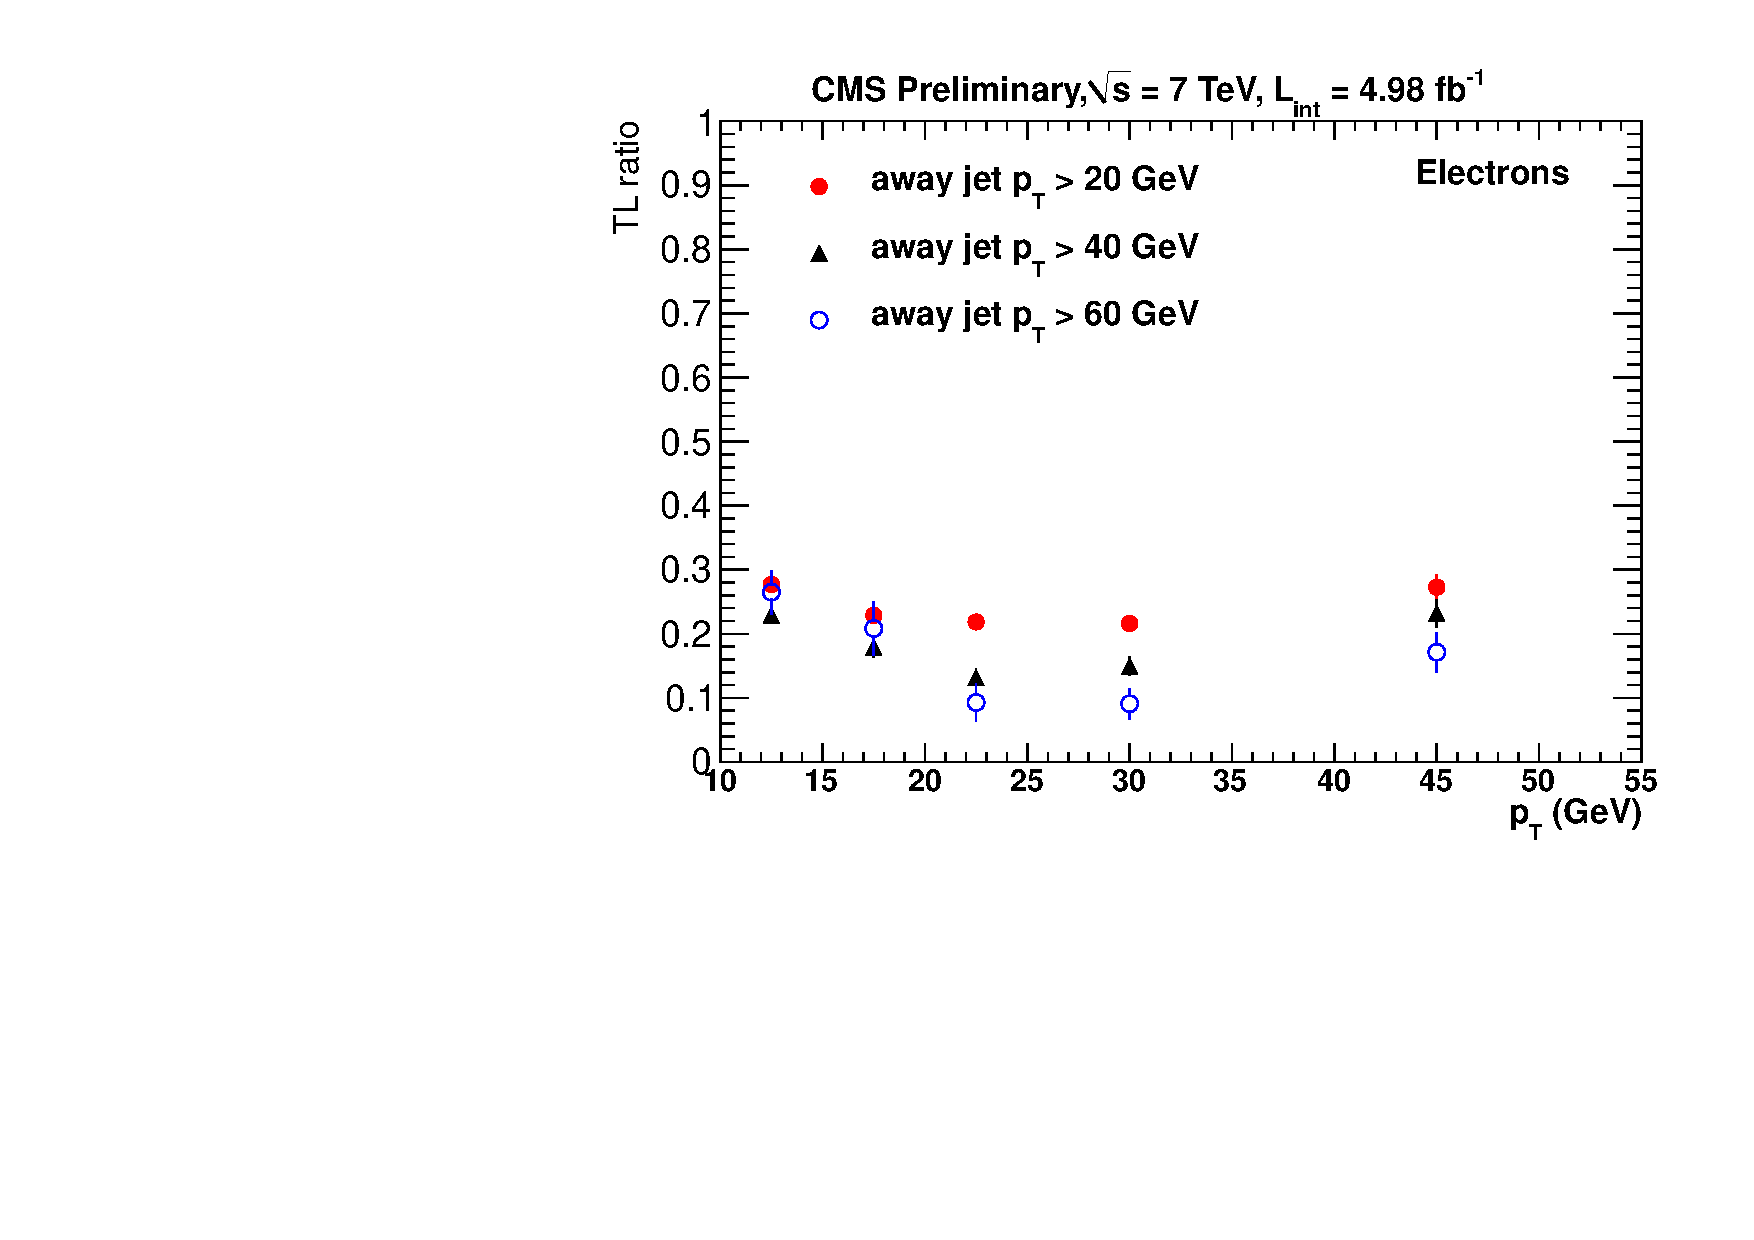
\includegraphics[width=0.48\linewidth]{figs/eleFRcaloIsoTrkIso_data_ptProj}
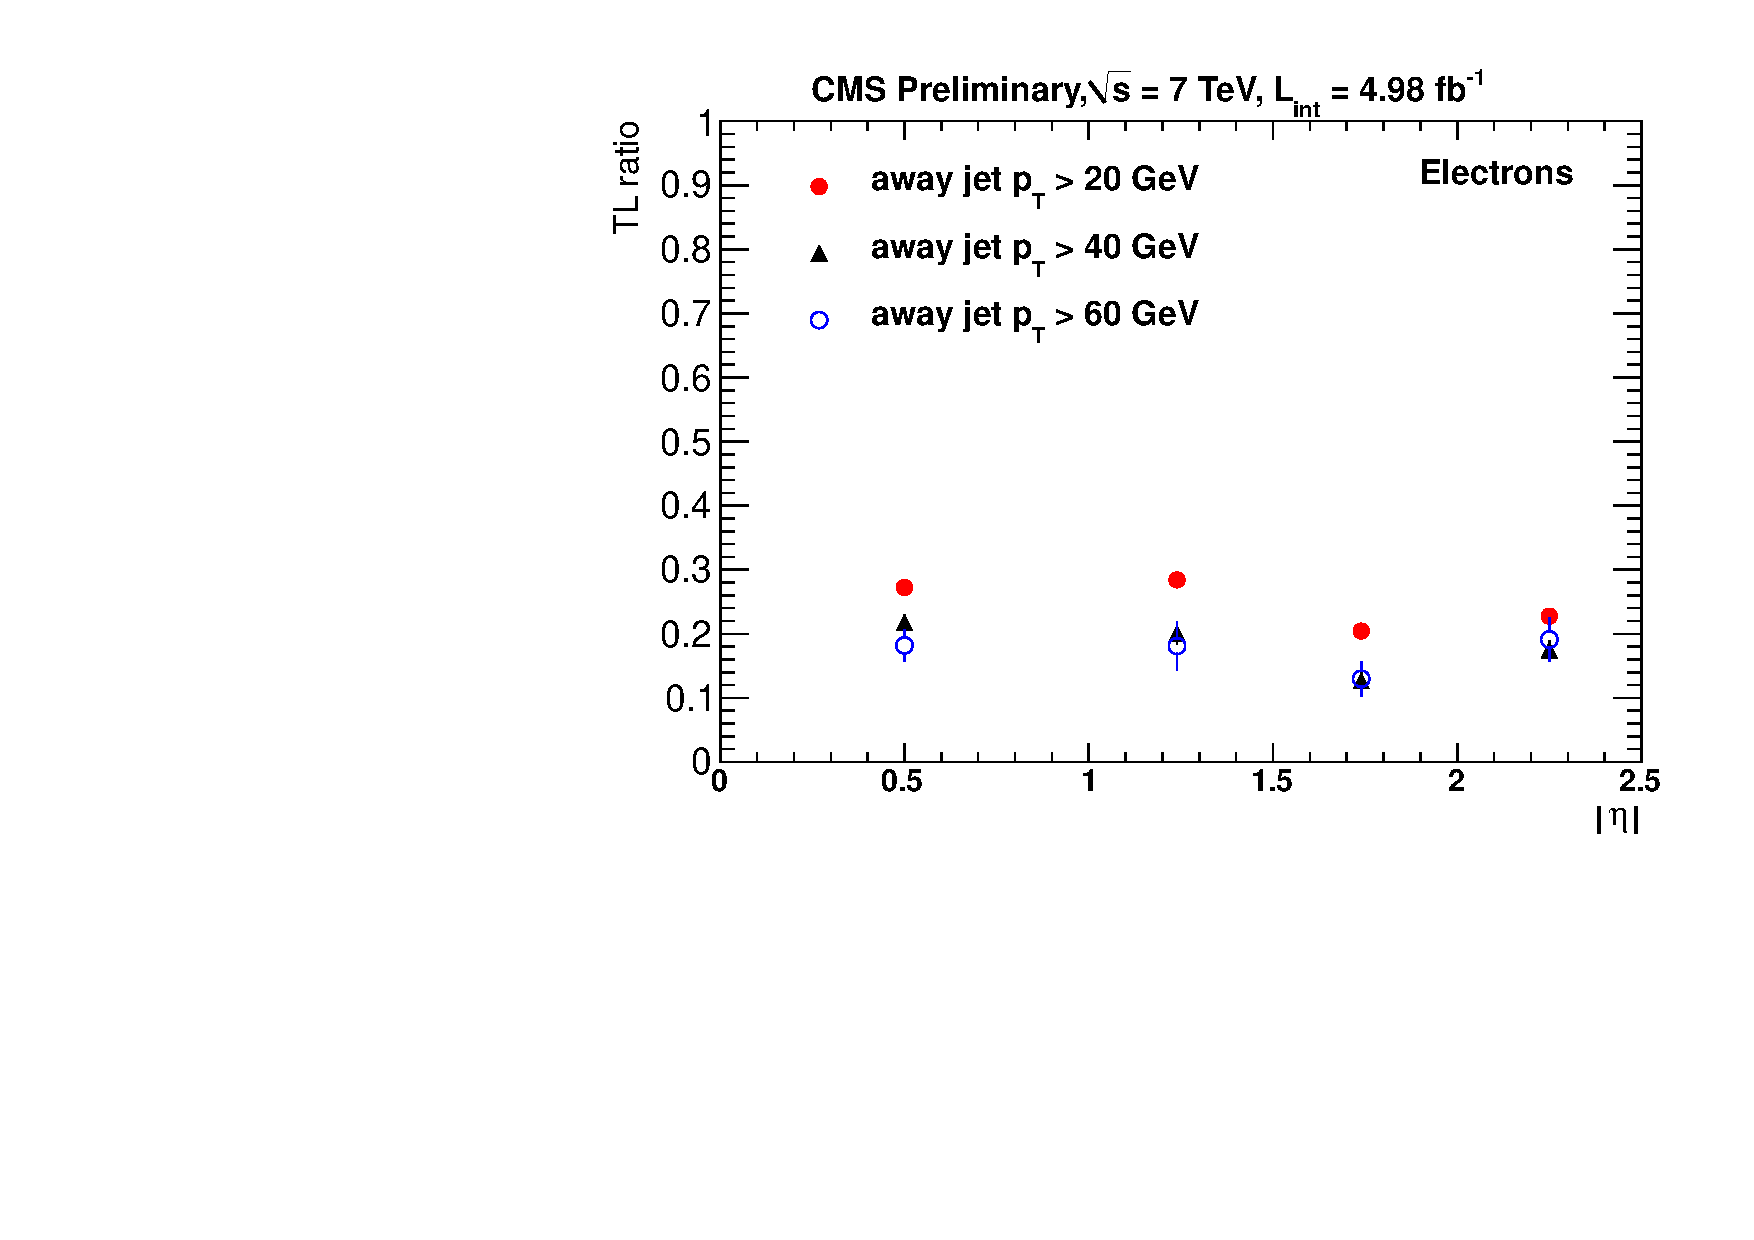
\includegraphics[width=0.48\linewidth]{figs/eleFRcaloIsoTrkIso_data_etaProj}\\
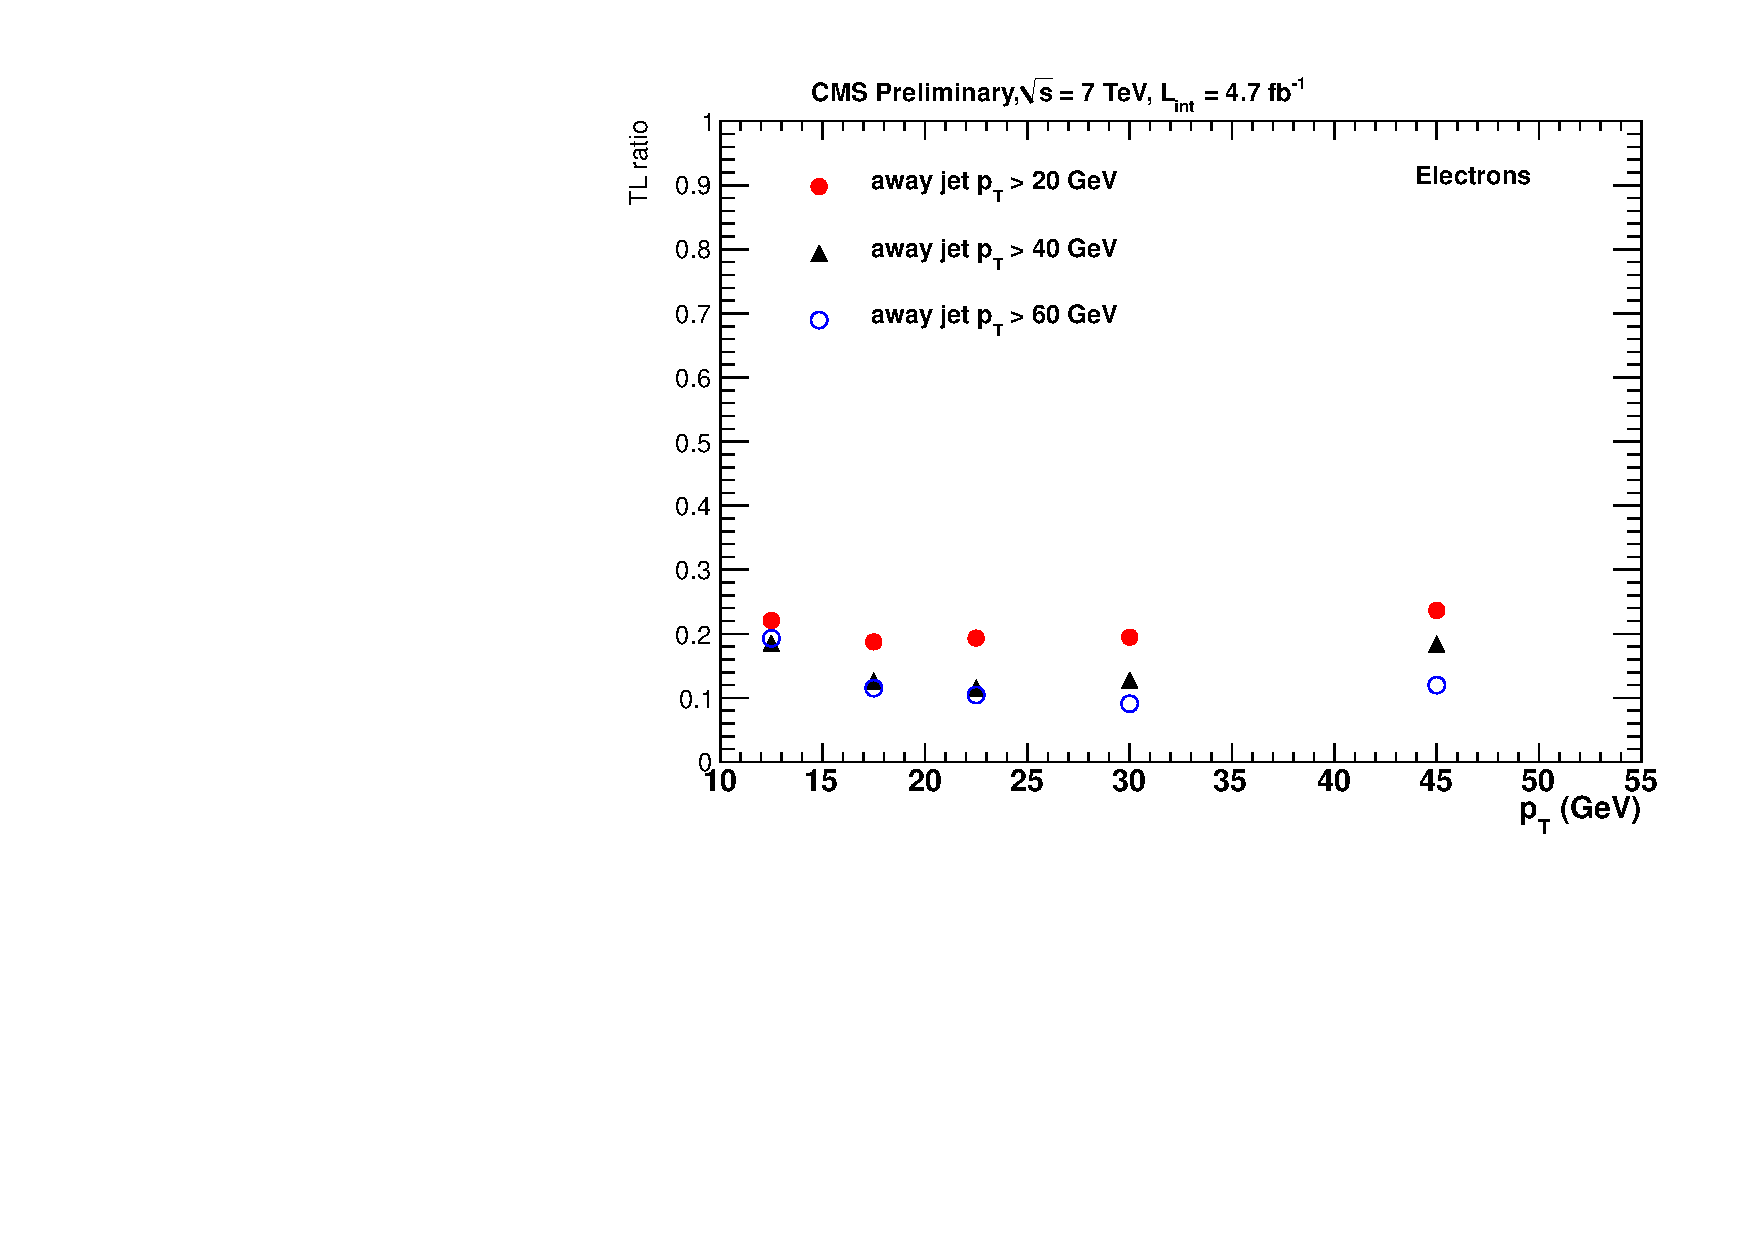
\includegraphics[width=0.48\linewidth]{figs/eleFRcaloIso_data_ptProj}
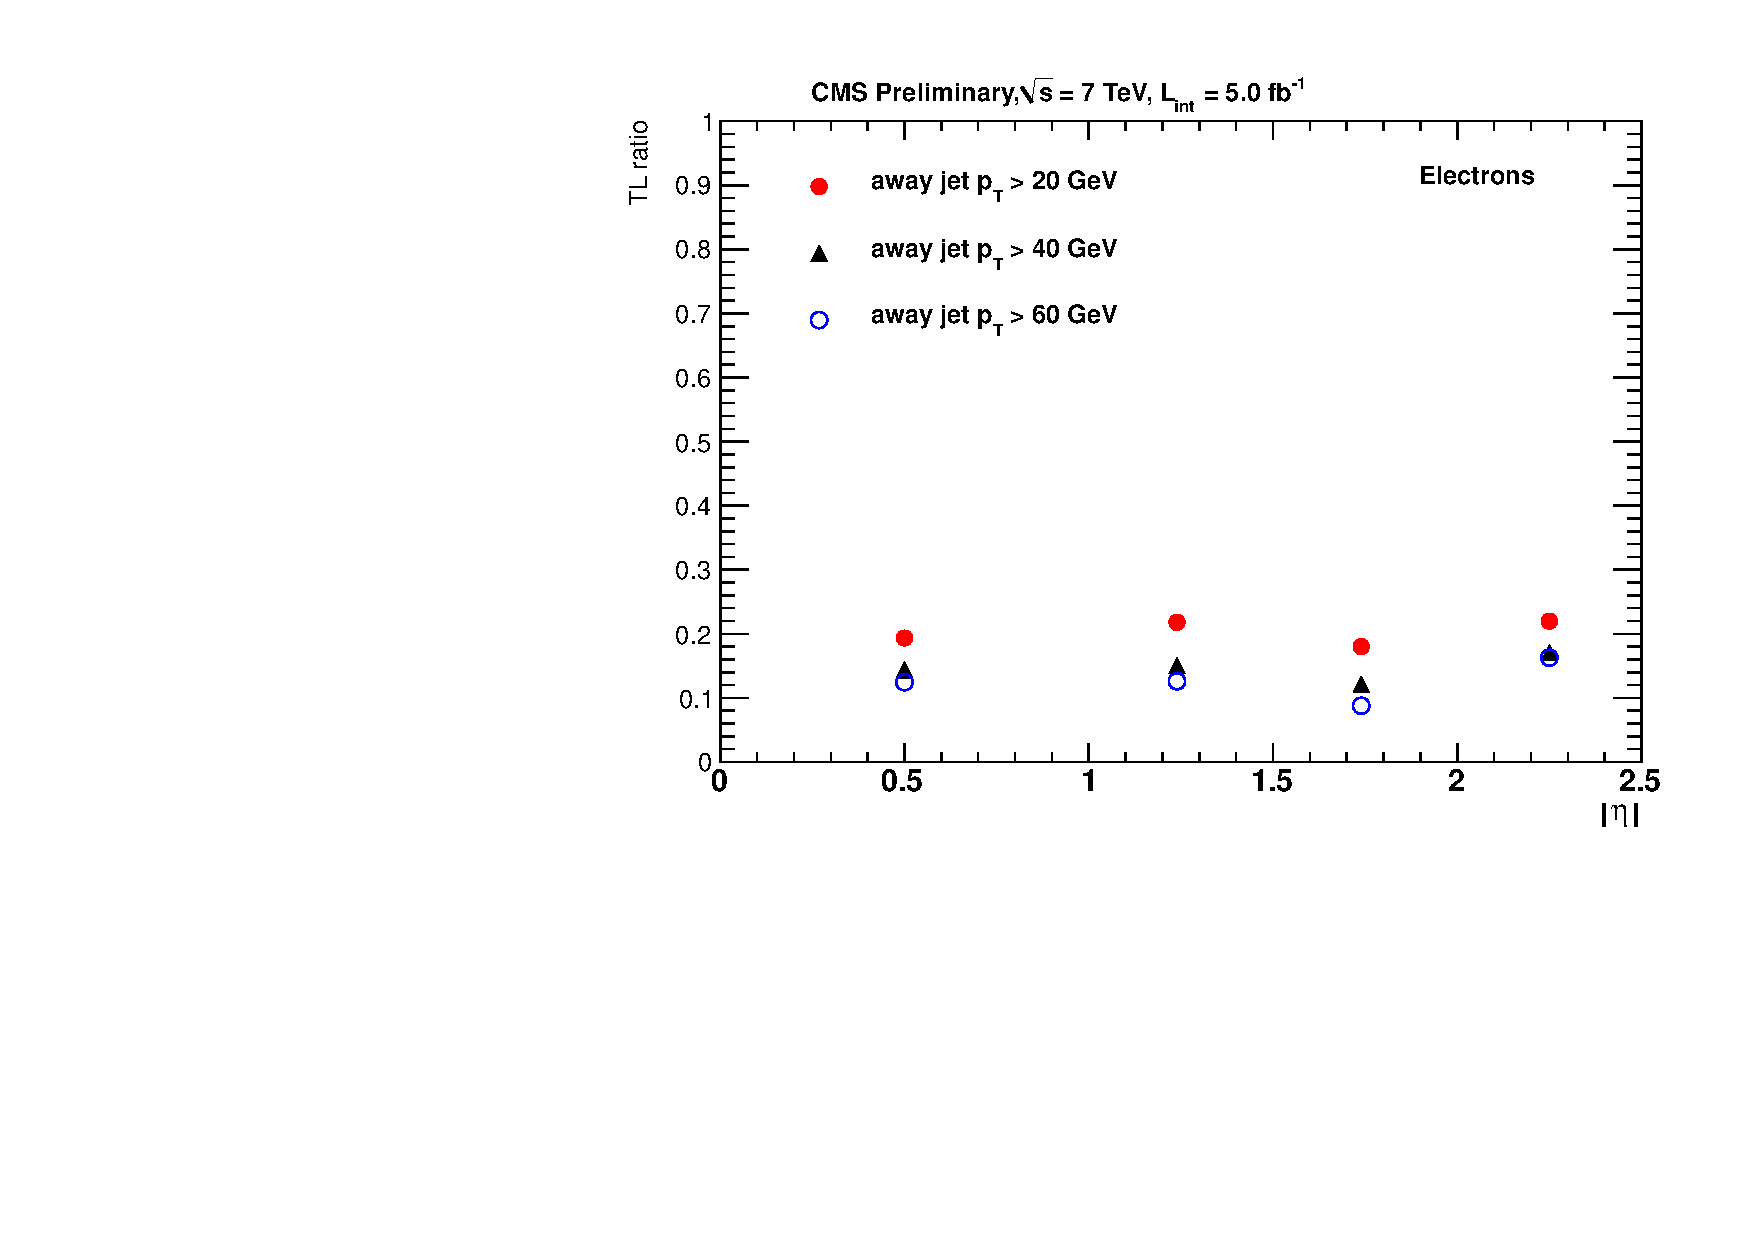
\includegraphics[width=0.48\linewidth]{figs/eleFRcaloIso_data_etaProj}\\
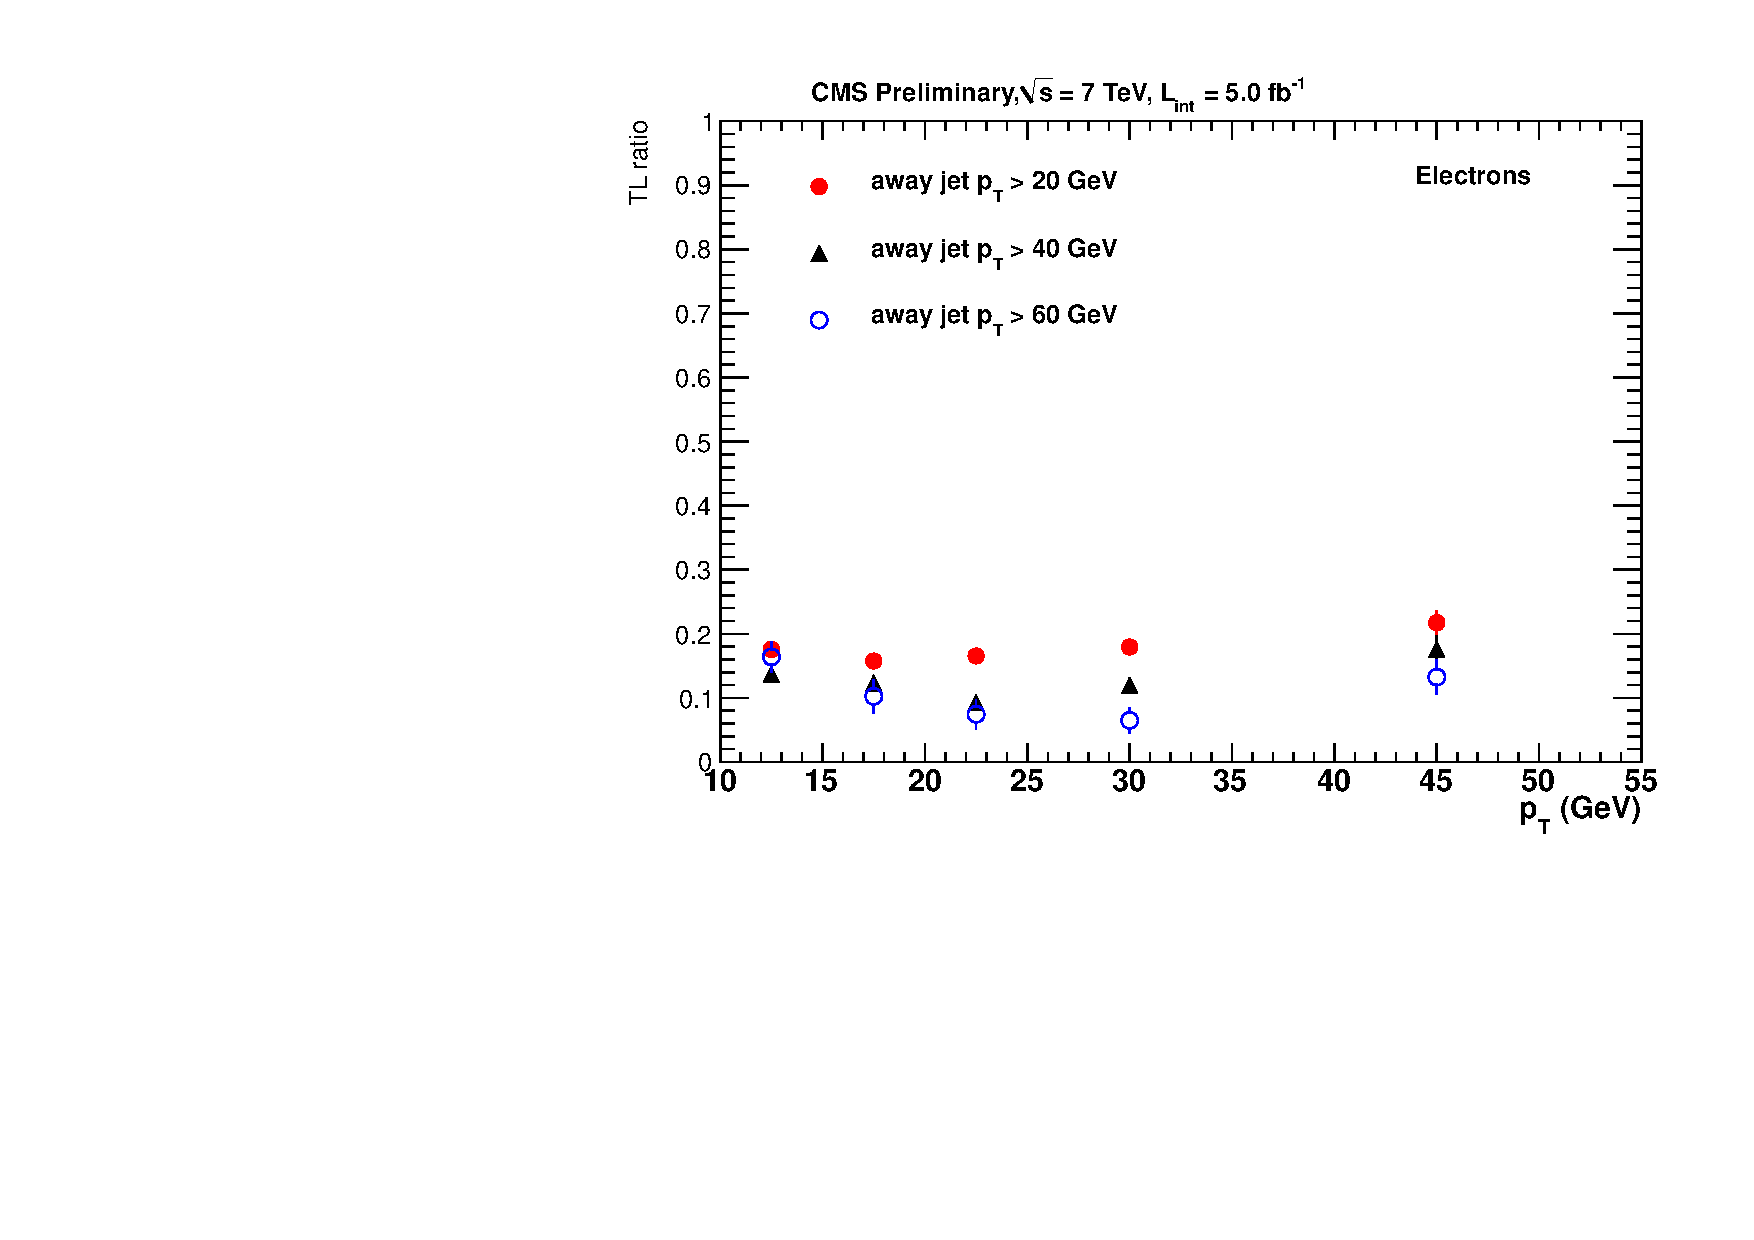
\includegraphics[width=0.48\linewidth]{figs/eleFRnoIso_data_ptProj}
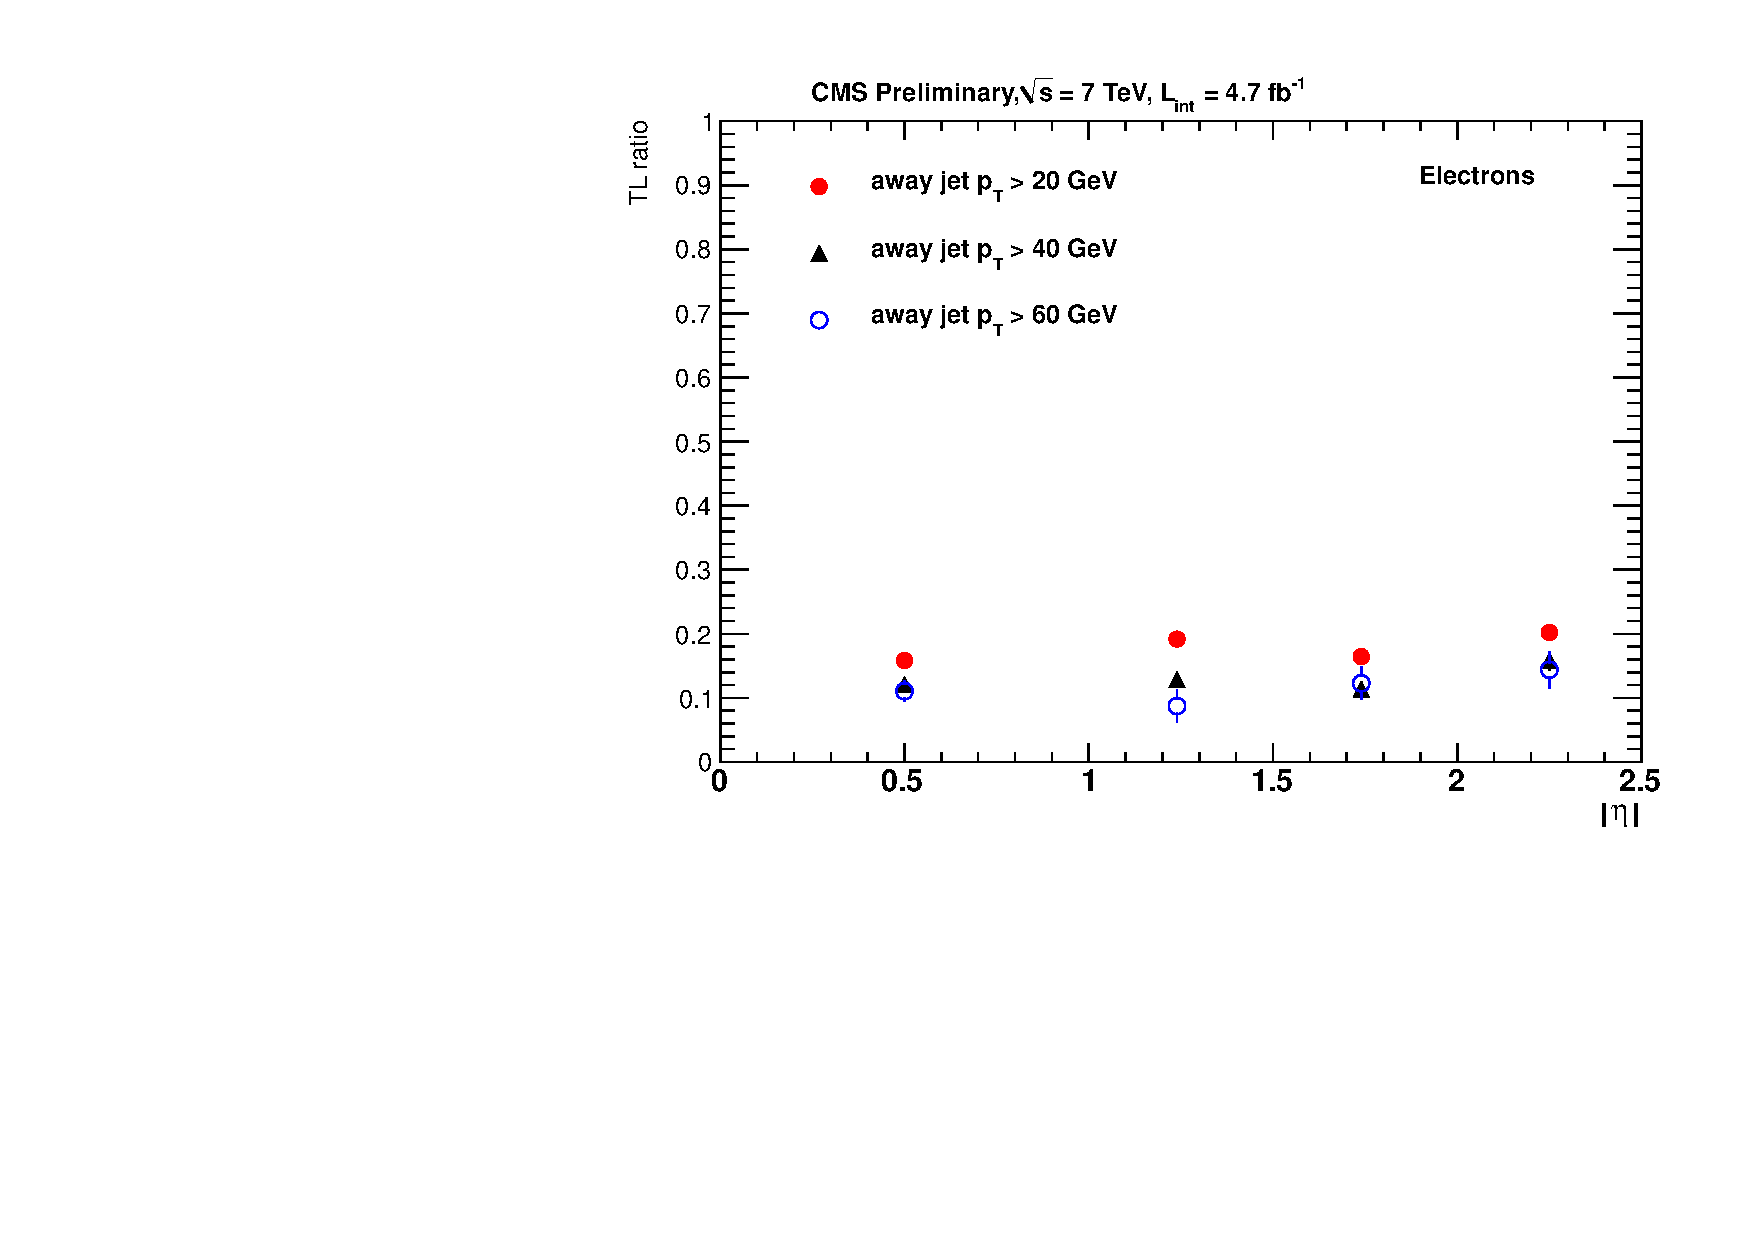
\includegraphics[width=0.48\linewidth]{figs/eleFRnoIso_data_etaProj}
\caption{\label{fig:frelectron}Electron fake rate projected on $\pt$ (left) and $|\eta|$ (right)
for electrons collected by the triggers with calorimeter and tracker isolation requirements (top), with a calorimeter isolation requirement (middle) and without an isolation requirement (bottom).
The fake rates are shown separately for measurements  with a requirement for an away jet \pt\ 
to be above 20~\GeV\ (red filled circles), 40~\GeV\ (black up triangles), and 60~\GeV\ (blue open circles).
}
\end{center}
\end{figure}

\clearpage

%Similar to the choice made in 2010 data analysis, we restrict the measurement of the fake rate
%to 35~\GeV\ (55~\GeV) for muons (electrons) in order to avoid the residual contribution from the W+jets
%and Z events.
%We find that the contribution from the W/Z production is small for electrons up to about 55~\GeV,
%as illustrated in Fig.~\ref{fig:freleptWZ} for data (left) and simulation (right), respectively.
%There is no significant contribution from the W events in the MC, which is supported by only marginal increase
%in the fake rate in data after the W suppression requirements are removed.
%For muons, since the selection did not change significantly, we refer to the corresponding figure 
%in~\cite{frmethod}.
%
%
%\begin{figure}[h]
%\begin{center}
%%\includegraphics[width=0.48\linewidth]{figs/}
%%\includegraphics[width=0.48\linewidth]{figs/}
%\caption{\label{fig:freleptWZ}Electron fake rate as a function of the electron $\pt$ measured
%for a range of selection enhancing the contribution from the W/Z events.
%The fake rate measured in data (left) is shown for the nominal measurement (circles) and for 
%a measurement without additional W suppression (squares) using triggers with a calorimeter isolation requirement.
%The electron fake rate measured in MC (right) is shown for the nominal measurement using 
%only QCD samples (circles), and that with the W sample included (up triangles),
%as well as for the selection without the W suppression measured in the QCD sample alone (squares)
%and that with the W sample included (down triangles).
%}
%\end{center}
%\end{figure}
%
%The following assumptions are made prior to applying the measured fake rates to the dilepton events.
%\begin{itemize}
%\item The fake rate per lepton is independent for the two leptons, e.g. 
%	to predict the fake contribution to an $e\mu$ final state we consider electron and muon fakes
%          separately, and add them up, assuming no correlations between the two estimates.
%\item We assume the lepton fake rate measurement in an inclusive QCD sample as 
%	described in~\cite{frmethod} represents the lepton fake rate  in the dilepton sample. 
%\end{itemize}

We test that the fake rates measured in QCD are applicable to the dilepton samples by performing closure
tests on simulated W+jets, \ttbar, and QCD samples.
The tests done on W+jets and \ttbar\ samples are done as follows
\begin{enumerate}
\item select events passing the baseline selections;
\item require that one lepton is matched to a leptonic W decay and the other (fake) lepton is not
matched to a leptonic W decay;
\item scale the number of fake leptons failing the full lepton selections and passing the FO selections
	by $FR/(1-FR)$ as a function of the fake lepton \pt\ and $|\eta|$ --- this is the prediction
	of the number of fakes passing full lepton selections;
\item compare the predicted and observed number of fake leptons.
\end{enumerate}
The prediction of the number of events with fakes gives a consistent overestimate for the \ttbar\ events
for both electrons and muons by approximately the same fraction of  $70\%$ of the observed value,
or, equivalently, the observed value differs from the prediction by approximately  40\% of the predicted value.
We attribute this to the difference in the underlying parton momenta in \ttbar\ and inclusive QCD events:
the momentum is generally higher in \ttbar\ events, which corresponds to a smaller effective fake rate.
We find that the prediction of the number of fakes gives a marginally significant underestimate 
for W+jets events.
The statistical uncertainty of this test  is much larger for muons than for electrons.
We expect this to happen if the jets initiating the fakes in W+jet events have a smaller momentum on average
compared to those used to extract the fake rate in QCD events.
Results of the closure tests on \ttbar\ and W+jet events passing the baseline selections of {\em high-\pt}
 dileptons are summarized in Table~\ref{tab:ttWjclosure}.
In addition to this, we have performed a closure test on the same-sign dimuon events in the QCD sample
(without any additional requirement on the number of jets or on \met):
we find that the number of expected events agrees with the  observed within statistical uncertainty of about 20\%.

\begin{table}[h]
\begin{center}
\begin{tabular}{lc|cc|cc}
\hline\hline
Sample	& result	&	\multicolumn{2}{|c}{ElectronFR}		& \multicolumn{2}{|c}{Muon FR}	\\
	&		&	$ee$		& $e\mu$		& $\mu\mu$	& $e\mu$	\\\hline
\ttbar	&	observed& $2.8\pm0.2$		& $4.2\pm0.2$		& $3.9\pm0.2$	& $4.0\pm0.2$	\\
	&predicted	& $4.9\pm0.4$		& $6.8\pm0.5$		& $7.2\pm 0.3$	& $6.5\pm 0.2$	\\ 
	&	ratio	& $1.8\pm0.2$		& $1.6\pm0.2$		& $1.8\pm 0.1$	& $1.6\pm 0.1$	\\ \hline
W+jets	&	observed& $<2.1$		& $8.4\pm4.2$		& \multicolumn{2}{|c}{$2.1\pm 2.1$} \\
	&  predicted	& $1.5\pm0.8$		& $3.4\pm1.4$		& \multicolumn{2}{|c}{$2.1\pm1.2$}	\\
	& ratio		& $<1.4$		& $0.4\pm0.3$		& \multicolumn{2}{|c}{$1.0\pm1.2$} \\
\hline\hline
\end{tabular}
\caption{\label{tab:ttWjclosure}Fake rate closure test on \ttbar\ and W+jets events for high-\pt\ dilepton
selections. 
The muon FR test in $e\mu$ is done with $\met>20~\GeV$.
The number of events is scaled to 1~\fbin.
Expcept for the test in \ttbar\ with electrons (done with jet $\pt>40~\GeV$), 
the results are reported for events with at least two jets with $\pt>30~\GeV$ (old selection), used to 
increase the number of events passing the selections.}
\end{center}
\end{table}

\newcommand{\nNoNu}{\ensuremath{N_{{n}\overline{n}}}}
\newcommand{\nNoNo}{\ensuremath{N_{\overline{n}\overline{n}}}}
\newcommand{\nNuNu}{\ensuremath{N_{{n}{n}}}}

%An estimate of the number of fake leptons in dilepton events passing full (numerator) selections
%is based on counts of dilepton events with two non-numerator \nNoNo, two numerator \nNuNu,
%and only one non-numerator object \nNoNu.
%Assuming \nNoNo\ is dominated by QCD (both leptons are fake), a relatively simple calculation
%leads to the following, neglecting much smaller terms.
%The QCD contribution to the signal sample $N^{QCD}_{nn}$ is given by
%$$
%N^{QCD}_{nn} = \sum_{i,j} \frac{FR_i FR_j}{(1-FR_i)(1-FR_j)} \nNoNo^{ij},
%$$
%where the indices $i, j$ correspond to the binning and flavor of corresponding non-numerator lepton objects.
%The contribution from one true and one fake lepton (e.g. $t\bar{t}$, single top, Wjets) 
%contribution in the signal sample $N^{W}_{nn}$ is given by
%$$
% N^{W,raw}_{nn} = \sum_{i} \frac{FR_i}{(1-FR_i)} \nNoNu^{i},
%$$
%$$
% N^{W}_{nn} =  N^{W,raw}_{nn} -  2 N^{QCD}_{nn}.
%$$
%
%The total prediction of the number of events with fake leptons is thus
%$$
% N^{fakes}_{nn} =  N^{W}_{nn} +  N^{QCD}_{nn}. 
%$$
The systematic uncertainty of $\pm 50\%$ per fake lepton is estimated for the fake rate method.
It is justified based on the closure tests and an understanding that the variation of the fake rate on
the jet momentum corresponds to the variation between the fakes from the ISR/FSR jets (like in W+jets),
and jets from the heavy final states (as in \ttbar).
We compute the contributions from QCD and W+jets and assign a 50\% systematic
uncertainty on the combined estimate.

We have neglected any "signal contamination". 
Signal contamination enters when there is a significant
source of two isolated leptons, with one or both failing the numerator cuts, but passing the denominator cuts
comprising  a significant fraction of the total number of \nNoNu\ or \nNoNo\ samples. 
Without an additional correction that can be easily applied,
a contribution from events with two real same-sign dileptons failing the numerator selections
 will overestimate the background contribution by approximately 3\% of the count of
the real same-sign dileptons passing the numerator selections.
Considering the size of the uncertainty on the background,
this effect can be safely ignored in the estimates 
of the fake leptons until the rate of same-sign dileptons passing the full
selections is at least an order of magnitude  higher than that expected
from fakes alone.
%As we see no evidence of any signal excess, we can safely ignore this.

%%%%%%%%%%
%%%%%%%%%%
%%%%%%%%%%
%%%%%%%%%%
%%%%%%%%%%
%%%%%%%%%%
%%%%%%%%%%
%%%%%%%%%%

\subsection{Data Driven prediction for charge mis-reconstruction backgrounds}
\label{sec:flips}

%%%%%%%%%%
%%%%%%%%%%

Following our original studies~\cite{sspaper2010} of the electron charge misreconstruction, 
we apply the requirement for electrons that all three charge measurements for a GSF electron agree. 
This dramatically reduces the rate of charge mismeasurement for electrons to the point where it 
is an almost negligible source of background, less than 10\% of the background due to fake leptons, 
as was shown in the 2010 analysis~\cite{sspaper2010}.
Even though this background is small, it is not necessarily well-reproduced in simulation.
We apply a data-driven method used in the previous analysis here.

The following steps are done:
\begin{enumerate}
\item Measure the probability for an electron to have its charge misreconstructed 
in bins of $|\eta |$ and $\pt$ using single electron gun Monte Carlo.
\item Use this probability and apply it to the opposite sign Z sample for a Z control sample 
defined as $76$\ GeV $ < m_{ll} < 106$\ GeV,  \met $ < 20$\ GeV,
and transverse mass $< 25$ GeV. 
Here transverse mass is calculated based on whichever lepton has higher $\pt$. 
Compare with the actual yield of double-charged Z candidates in that region to establish validity of the approach.
\item If the expected and observed yields agree reasonably well in the previous step, continue using
	the probability measured in the first step and use the discrepancy as a systematic uncertainty.
\item Then apply this probability to all the electrons in opposite sign dilepton events that pass the selection. 
	This produces the data driven charge flip  prediction shown in the tables in Section~\ref{sec:yields}. 
\item The lepton $p_T$ distributions of leptons from top is slightly harder than that for leptons from Z. The above
test thus does not fully sample the lepton spectrum for our background sample. We assign an additional systematics
to account for this effect.
\end{enumerate}

Figure~\ref{fig:flipvsptOrEta} shows the $\pt$ (left) and $|\eta |$ (right) projections of 
the charge mismeasurement probability  from single electron gun Monte Carlo.
The same function is applied to data and MC.  
As seen in Fig.~\ref{fig:flipvsptOrEta} (right), the charge mismeasurement probability
did not change substantially in the samples used for the previous analysis, as well as for the Spring11 and Summer11
simulation.

\begin{figure}[h]
\begin{center}
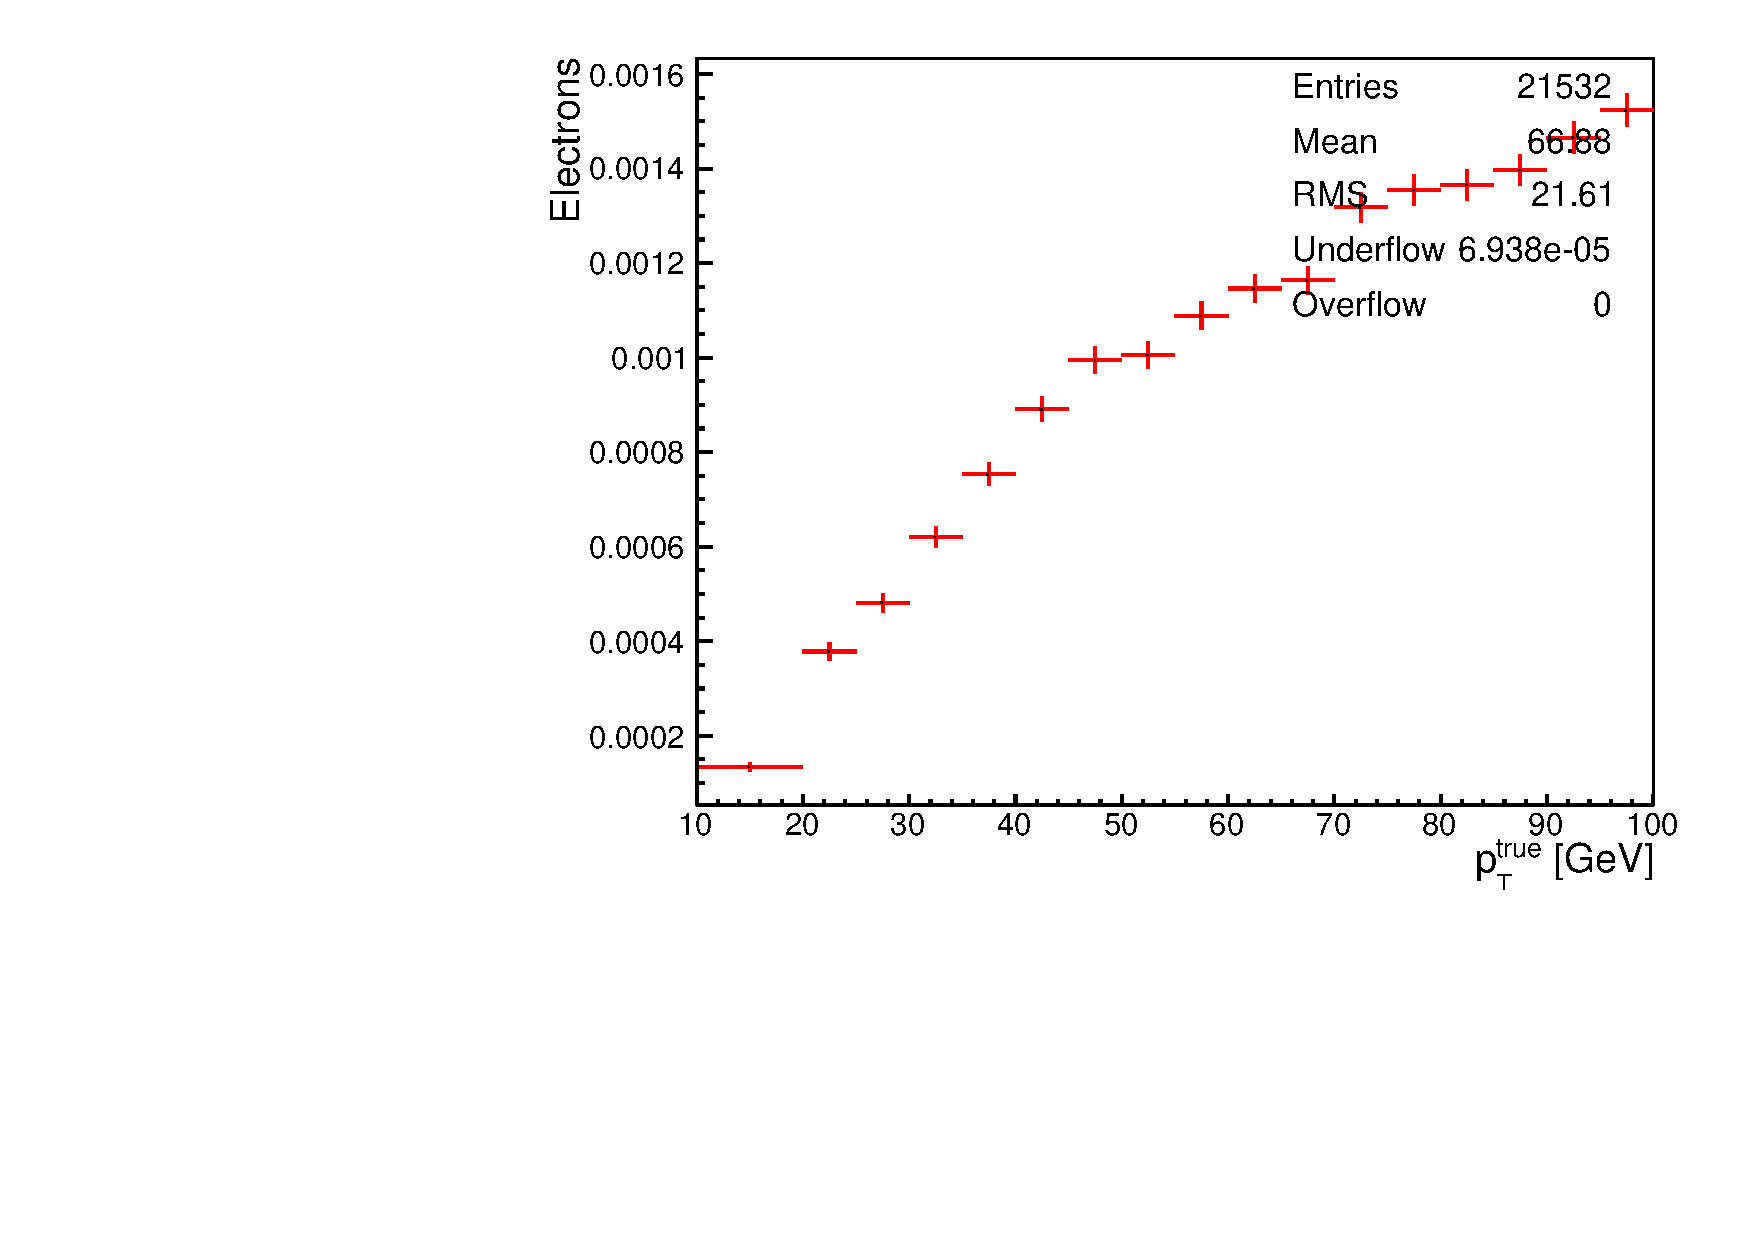
\includegraphics[width=0.47\linewidth]{figs/flipRate2011VsPt}
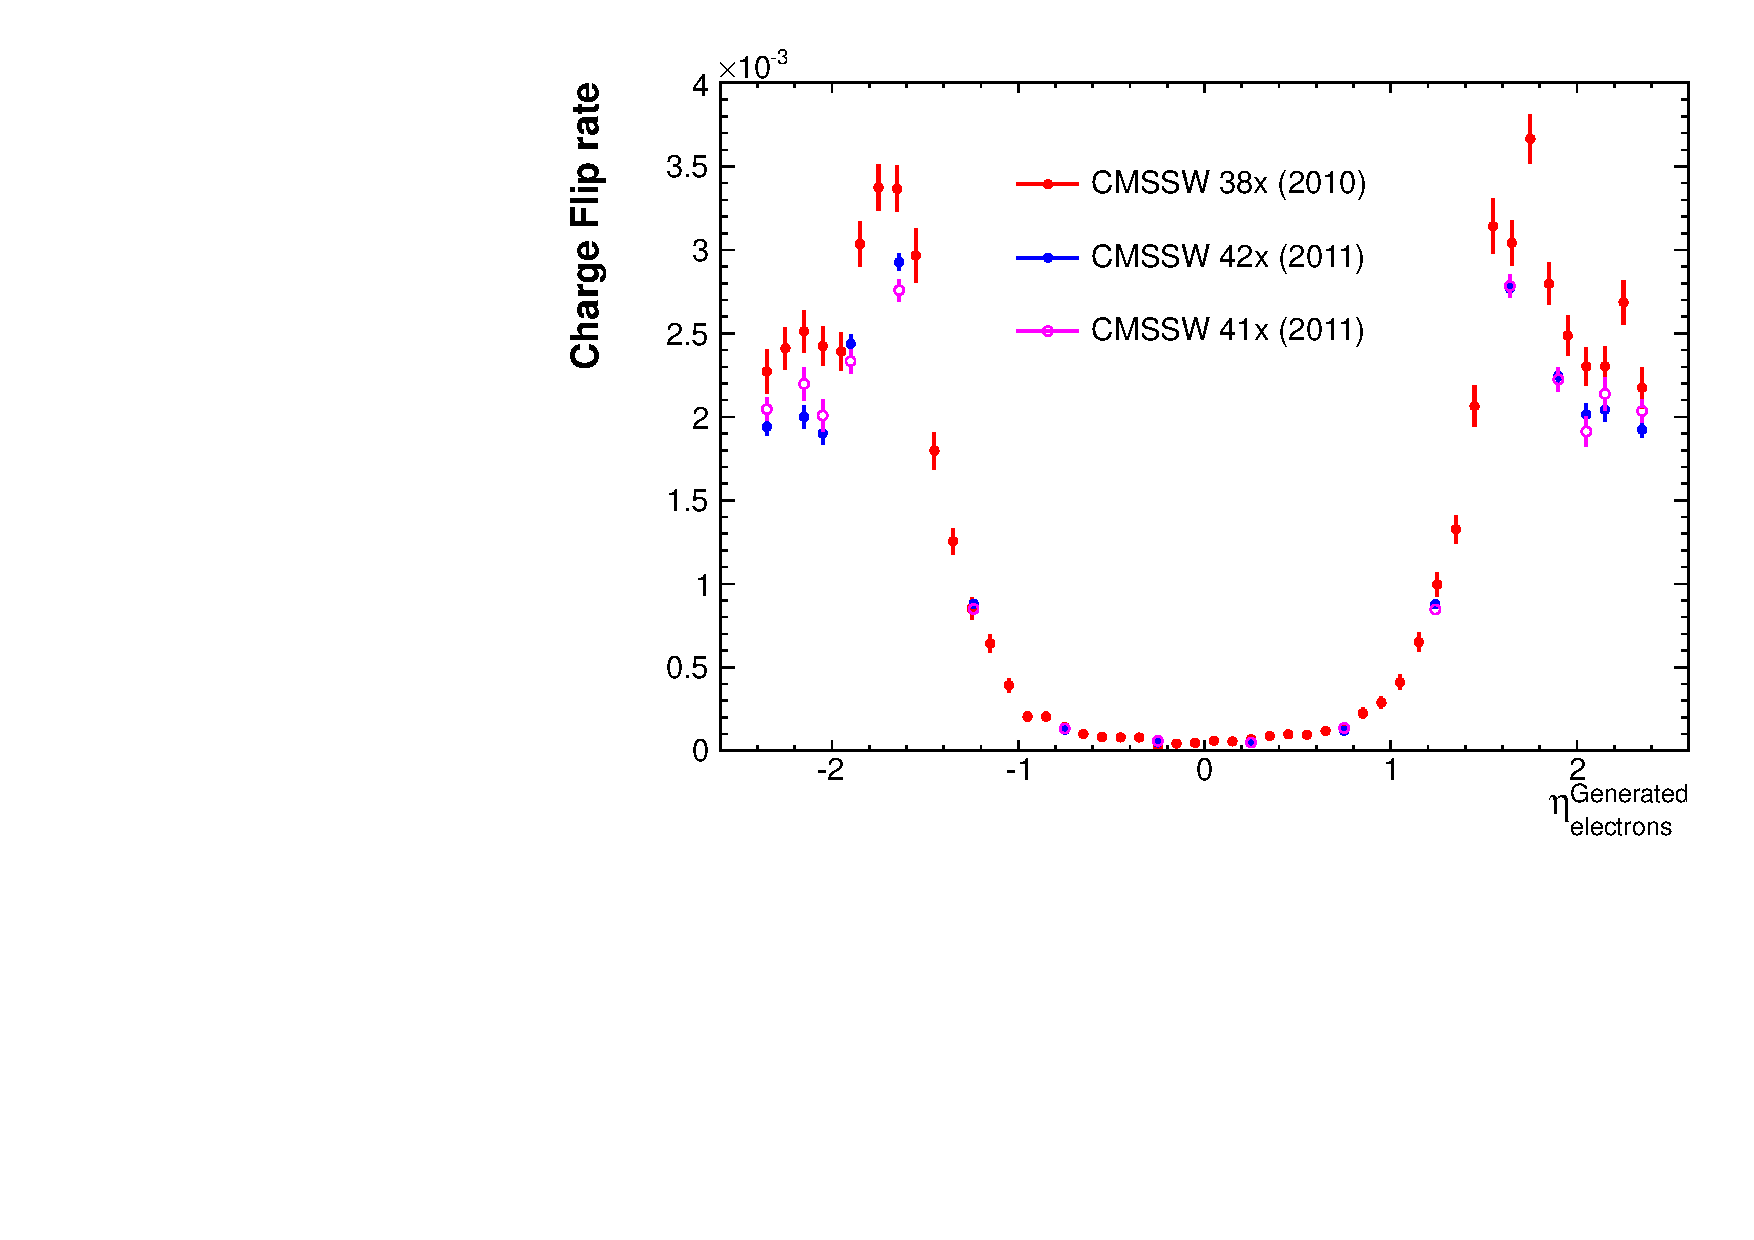
\includegraphics[width=0.47\linewidth]{figs/flipRate2011PAS}
\caption{\label{fig:flipvsptOrEta}Charge mismeasurement probability from single electron gun MC
shown in projections on $\pt$ (left) and $\eta$ (right).
The projection on $\eta$ also shows the distributions for the charge mismeasurement probability
in 2010 analysis (red), current definition (blue), and that in the older (Spring11-like) MC sample.}
\end{center}
\end{figure}

We find 390 events with same-sign electron pairs in data in the Z control region.
This needs to be compared with the sum of the expected same-sign events as estimated from
opposite-sign dielectrons, $359.7\pm4.1$, plus a contribution from fakes, $11\pm 6$.
The number of events expected directly from simulation is  $469\pm 11$.
The same-sign dielectron mass distribution observed in data is compared to the expectation from
simulation in Fig.~\ref{fig:flipZee}.
These comparisons are consistent within statistics.
The uncertainty is taken to be 20\% to account for kinematic differences between leptons from Drell-Yan events and top pairs, the latter expected to be the dominant source of background events for this analysis.
%Based on these observations we assign a correction factor of $1.2\pm0.2$ to 
%the expected number of same-sign dielectron
%events obtained using the opposite-sign dielectron samples.
%The scale factor corresponds to the relative difference between $121\pm11({\rm stat.})\pm 4({\rm syst})$ 
%and $100\pm 0.3$, the uncertainty is taken to be 20\% to account in addition for potential effects
%not covered by this test with Z events.


\begin{figure}[h]
\begin{center}
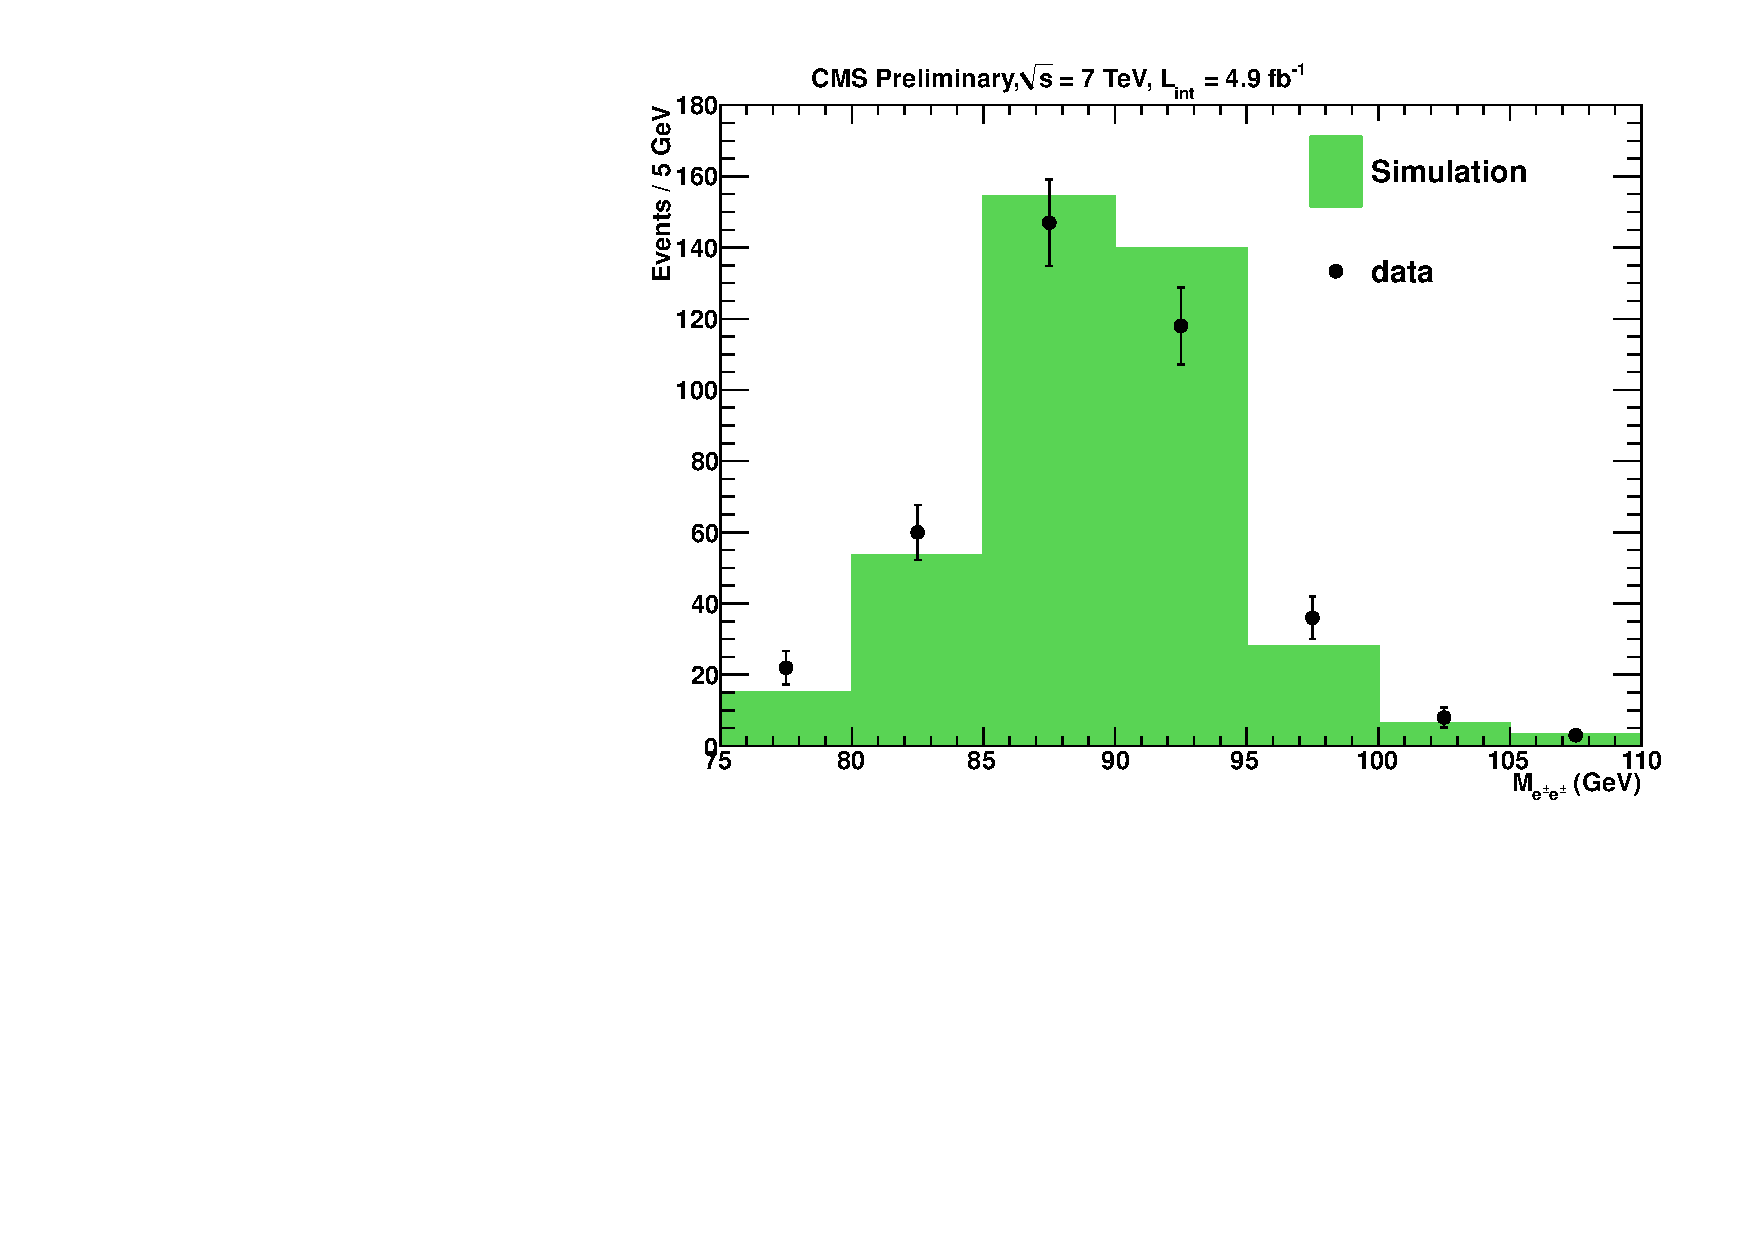
\includegraphics[width=0.8\linewidth]{figs/qflip_data_mc_comp}
\caption{\label{fig:flipZee}
Same sign $ee$ invariant mass distribution compared with $Z \to ee$ Monte Carlo expectations.
Cuts on missing transverse energy $<$ 20 GeV and transverse mass
$<$ 25 GeV have been applied to reduce backgrounds from $W +$ jets.
The highest $\pt$ lepton has been used in the calculation of the transverse  mass.}
\end{center}
\end{figure}









